\mysection{HW/SW-Components}\label{component}

A real-time embedded system consists of components, that provide the service capacity of the resources to the event streams, in order to give them the supplies they need for
executing their tasks.
Whenever an event stream now arrives at a computational or communicational component, an application task is interpreted and executed~\cite{wan:06}.
This processing usually leads to changes in the event arrival and service curves.
So how can we derive the properties of the outgoing streams \(\alpha'\) and \(\beta'\) from the properties of the incoming streams \(\alpha\) and \(\beta\)?

Let's suppose we have a simple system with only one single event stream arrival curve \(\alpha\) and one resource with service capacity \(\beta\) like in \autoref{fig:single_GPC}~\cite{ver}~\cite{thi:00}.

\begin{figure}
    \centering
    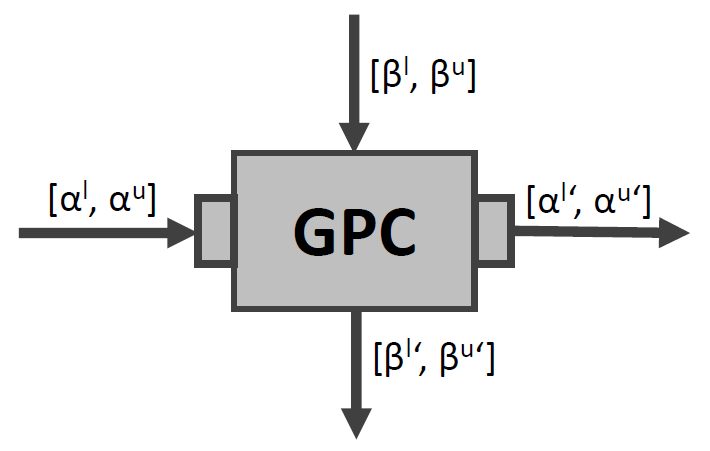
\includegraphics[width=0.7\columnwidth]{graphics/single_GPC.png}
    \caption{Single GPC with its incoming and outgoing streams}\label{fig:single_GPC}
\end{figure}

The pair of output arrival curves describes the event rates after this processing step, while the pair of output service curves describes the remaining service capacity~\cite{wan:06}.
The relations between \(\alpha, \beta, \alpha' \text{ and } \beta'\) and thereby the values of \(\alpha' \text {and } \beta'\) depend on the processing semantics of the component.
In general, they can be modeled as
\[ \alpha' = f_\alpha (\alpha, \beta)\] 
\[\beta' = f_\beta (\alpha, \beta) \]
where the function \textbf{f} is given for each component specifically and
depends on the processing semantics of the modeled component~\cite{wan:06}.
These processing semantics need to be provided in the application or resource description.

In the framework of MPA we are mostly working with abstract components.
Here the input and output streams are no concrete traces, but always just upper and lower borders for possible traces, like for example \(\alpha' = [\alpha'^{\, u}, \alpha'^{\, l}]\)~\cite{wan:06}.

Greedy processing components (\textbf{GPC}) are a common example for such components in real-time embedded systems.
A GPC is triggered by an incoming event, directly instantiates a task and then processes the event, and thereby its task, in a greedy fashion
in first-in-first-out order~\cite{cho:08}.
Of course this process is restricted by the resource availability \(\beta\).
The main advantage of using GPCs is, that we can easily compute the semantics of the component using the min/max-plus algebra (see \autoref{minMaxPlus})~\cite{wan:06}.
Thus, we will from now on assume that all of the components in this paper are GPC.

With a GPC the resulting event streams are~\cite{wan:06}:
\[\alpha'^{\, u} = \min \left\{ (\alpha^{u} \otimes \beta ^{\, u}) \oslash \beta^{\, l}, \beta^{\, u} \right\} \]
\[\alpha'^{\, l} = \min \left\{ (\alpha^{l} \oslash \beta ^{\, u}) \otimes \beta^{\, l}, \beta^{\, l} \right\} \]
While the remaining service capacities are:
\[\beta \, ^{\prime\, u} = (\beta ^{\, u} - \alpha ^{l}) \overline{\oslash} 0 \]
\[\beta \, ^{\prime\, l} = (\beta ^{\, l} - \alpha ^{u}) \overline{\otimes} 0 \]